\documentclass[a4]{article}
\pagestyle{myheadings}

%%%%%%%%%%%%%%%%%%%
% Packages/Macros %
%%%%%%%%%%%%%%%%%%%
\usepackage{mathrsfs}


\usepackage{fancyhdr}
\pagestyle{fancy}
\lhead{}
\chead{}
\rhead{}
\lfoot{}
\cfoot{} 
\rfoot{\normalsize\thepage}
\renewcommand{\headrulewidth}{0pt}
\renewcommand{\footrulewidth}{0pt}
\newcommand{\RomanNumeralCaps}[1]
    {\MakeUppercase{\romannumeral #1}}

\usepackage{amssymb,latexsym}  % Standard packages
\usepackage[utf8]{inputenc}
\usepackage[russian]{babel}
\usepackage{MnSymbol}
\usepackage{mathrsfs}
\usepackage{amsmath,amsthm}
\usepackage{indentfirst}
\usepackage{graphicx}%,vmargin}
\usepackage{graphicx}
\graphicspath{{pictures/}} 
\usepackage{verbatim}
\usepackage{color}
\usepackage{color,colortbl}
\usepackage[nottoc,numbib]{tocbibind}
\usepackage{float}
\usepackage{multirow}
\usepackage{hhline}

\usepackage{listings}
\definecolor{codegreen}{rgb}{0,0.6,0}
\definecolor{codegray}{rgb}{1,1,1}
\definecolor{codepurple}{rgb}{0.58,0,0.82}
\definecolor{backcolour}{rgb}{0.95,0.95,0.92}
 
\lstdefinestyle{mystyle}{
    backgroundcolor=\color{backcolour},   
    commentstyle=\color{codegreen},
    keywordstyle=\color{magenta},
    numberstyle=\tiny\color{codegray},
    stringstyle=\color{codepurple},
    basicstyle=\footnotesize,
    breakatwhitespace=false,         
    breaklines=true,                 
    captionpos=b,                    
    keepspaces=true,                 
    numbers=left,                    
    numbersep=5pt,                  
    showspaces=false,                
    showstringspaces=false,
    showtabs=false,                  
    tabsize=2
}
 
\lstset{style=mystyle}

\usepackage{url}
\urldef\myurl\url{foo%.com}
\def\UrlBreaks{\do\/\do-}
\usepackage{breakurl}
\Urlmuskip=0mu plus 1mu



\DeclareGraphicsExtensions{.pdf,.png,.jpg}% -- настройка картинок

\usepackage{epigraph} %%% to make inspirational quotes.
\usepackage[all]{xy} %for XyPic'a
\usepackage{color} 
\usepackage{amscd} %для коммутативных диграмм
%\usepackage[colorlinks,urlcolor=red]{hyperref}

%\renewcommand{\baselinestretch}{1.5}
%\sloppy
%\usepackage{listings}
%\lstset{numbers=left}
%\setmarginsrb{2cm}{1.5cm}{1cm}{1.5cm}{0pt}{0mm}{0pt}{13mm}


\newtheorem{Lemma}{Лемма}[section]
\newtheorem{Proposition}{Предложение}[section]
\newtheorem{Theorem}{Теорема}[section]
\newtheorem{Corollary}{Следствие}[section]
\newtheorem{Remark}{Замечание}[section]
\newtheorem{Definition}{Определение}[section]
\newtheorem{Designations}{Обозначение}[section]




%%%%%%%%%%%%%%%%%%%%%%% 
%Подготовка оглавления% 
%%%%%%%%%%%%%%%%%%%%%%% 
\usepackage[titles]{tocloft}
\renewcommand{\cftdotsep}{2} %частота точек
\renewcommand\cftsecleader{\cftdotfill{\cftdotsep}}
\renewcommand{\cfttoctitlefont}{\hspace{0.38\textwidth} \LARGE\bfseries} 
\renewcommand{\cftsecaftersnum}{.}
\renewcommand{\cftsubsecaftersnum}{.}
\renewcommand{\cftbeforetoctitleskip}{-1em} 
\renewcommand{\cftaftertoctitle}{\mbox{}\hfill \\ \mbox{}\hfill{\footnotesize Стр.}\vspace{-0.5em}} 
%\renewcommand{\cftchapfont}{\normalsize\bfseries \MakeUppercase{\chaptername} } 
%\renewcommand{\cftsecfont}{\hspace{1pt}} 
\renewcommand{\cftsubsecfont}{\hspace{1pt}} 
%\renewcommand{\cftbeforechapskip}{1em} 
\renewcommand{\cftparskip}{3mm} %определяет величину отступа в оглавлении
\setcounter{tocdepth}{5} 
\renewcommand{\listoffigures}{\begingroup %добавляем номер в список иллюстраций
\tocsection
\tocfile{\listfigurename}{lof}
\endgroup}
\renewcommand{\listoftables}{\begingroup %добавляем номер в список иллюстраций
\tocsection
\tocfile{\listtablename}{lot}
\endgroup}


%\renewcommand{\thelikesection}{(\roman{likesection})}
%%%%%%%%%%%
% Margins %
%%%%%%%%%%%
\addtolength{\textwidth}{0.7in}
\textheight=630pt
\addtolength{\evensidemargin}{-0.4in}
\addtolength{\oddsidemargin}{-0.4in}
\addtolength{\topmargin}{-0.4in}

%%%%%%%%%%%%%%%%%%%%%%%%%%%%%%%%%%%
%%%%%%Переопределение chapter%%%%%% 
%%%%%%%%%%%%%%%%%%%%%%%%%%%%%%%%%%%
\newcommand{\empline}{\mbox{}\newline} 
\newcommand{\likechapterheading}[1]{ 
\begin{center} 
\textbf{\MakeUppercase{#1}} 
\end{center} 
\empline} 

%%%%%%%Запиливание переопределённого chapter в оглавление%%%%%% 
\makeatletter 
\renewcommand{\@dotsep}{2} 
\newcommand{\l@likechapter}[2]{{\bfseries\@dottedtocline{0}{0pt}{0pt}{#1}{#2}}} 
\makeatother 
\newcommand{\likechapter}[1]{ 
\likechapterheading{#1} 
\addcontentsline{toc}{likechapter}{\MakeUppercase{#1}}} 




\usepackage{xcolor}
\usepackage{hyperref}
\definecolor{linkcolor}{HTML}{000000} % цвет ссылок
\definecolor{urlcolor}{HTML}{3643FF} % цвет гиперссылок
 
\hypersetup{pdfstartview=FitH,  linkcolor=linkcolor,urlcolor=urlcolor, colorlinks=true}

%%%%%%%%%%%%
% Document %
%%%%%%%%%%%%

%%%%%%%%%%%%%%%%%%%%%%%%%%%%%
%%%%%%главы -- section*%%%%%%
%%%%section -- subsection%%%%
%subsection -- subsubsection%
%%%%%%%%%%%%%%%%%%%%%%%%%%%%%
\def \newstr {\medskip \par \noindent} 



\begin{document}
\newcolumntype{g}{>{\columncolor{codegray}}c}



\def\contentsname{\LARGE{Содержание}}
\thispagestyle{empty}

	\begin{center} 
		\vspace{2cm} 
		{\Large \sc Санкт-Петербургский Политехнический Университет}\\
		\vspace{2mm}
		{\Large\sc им. Петра Великого}\\
		\vspace{1cm}
		{\large \sc Институт прикладной математики и механики\\ 
			\vspace{0.5mm}
			\textsc{}}\\ 
		\vspace{0.5mm}
		{\large\sc Кафедра $"$Прикладная математика$"$}\\
		\vspace{15mm}
		
		
		{\sc \textbf{Отчёт по\\
				Лабораторным работам № 5-8\\
				по дисциплине\\
				"Математическая статистика"}
			\vspace{6mm}
			
		}
		\vspace*{2mm}
		
		
		\begin{flushleft}
			\vspace{4cm}
			\sc Выполнил студент:\\
			\sc Мальцов Дмитрий Дмитриевич\\
			\sc группа: 3630102/70401\\
			\vspace{1cm}
			\sc Проверил:\\
			\sc к.ф-м.н., доцент\\
			\sc Баженов Александр Николаевич
			\vspace{20mm}
		\end{flushleft}
	\end{center} 
	\begin{center}
		\vfill {\large\textsc{Санкт-Петербург}}\\ 
		2020 год
	\end{center}


\newpage
\pagestyle{plain}



\newpage
\tableofcontents{}
\newpage
\listoffigures{}
\listoftables{}
\newpage

\section{Постановка задачи}

\subsection{Вычисление коэффициента корреляции}

Необходимо построить выборки объёмом $20, 60, 100, 1000$ для двумерного нормального распределения с коэффициентами корреляции $\rho = 0, 0.5, 0.9$

Вычислить коэффициент корреляции Пирсона, Спирмана и квадрантный коэффициент корреляции для каждой выборки. Эти же вычисления повторить для смеси двумерных нормальных распределений: 
\begin{equation}
    f(x,y) = 0.9N(x,y,0,0,1,1,0.9)+0.1N(x,y,0,0,10,10,-0.9)
\end{equation}
На графике изобразить точки выборки и эллипс равновероятности.

\subsection{Оценки линий регрессии}
Необходимо найти оценки линейной регрессии $y_i=a+bx_i+e_i,$ используя $20$ точек отрезка $[-1.8;\;2]$ с равномерным шагом $0.2.$ Ошибку $e_i$ считать нормально распределённой с параметрами $(0,\;1).$ В качестве эталонной зависимости взять $y_i=2+2x_i+e_i.$ При построении оценок коэффициентов использовать два критерия: критерий наименьших квадратов и критерий наименьших модулей.
Проделать то же самое для выборки, у которой в значении $y_1$ и $y_{20}$ вносятся возмущения $10$ и $-10$ соответственно.

\subsection{Точечная оценка параметров распределения}

Необходимо сгенерировать выборку объемом $100$ элементов для нормального распределения $N(x;0,1).$ По сгенерированной выборке оценить параметры $\mu$ и $\sigma$ нормального закона методом максимального правдоподобия. В качестве основной гипотезы $H_0$ будем считать, что сгенерированное распределение имеет вид $N(x,\overset{\wedge}{\mu},\overset{\wedge}{\sigma} ).$ Проверить основную гипотезу, используя критерий согласия $\chi$. В качестве ровня значимости взять $\alpha=0,05.$ Проверить гипотизу о нормальности исходного распределения для выборки из распределения Лапласа размером $ n = 25 .$ Привести таблицы вычислений $\chi^2.$
\subsection{Интервальные оценки параметров распределения}

Для двух выборок $20$ и $100$ элементов, сгенерированных согласно нормальному закону $N(x,0,1),$ для параметров масштаба и положения построить асимптотически нормальные интервальные оценки на основе точечных оценок метода максимального правдоподобия и классические интервальные оценки на основе статистик $\chi^2$ и Стьюдента. В качестве параметра надёжности взять $\gamma = 0.95.$ 

\section{Теория}

\subsection{Вычисление коэффициента корреляции}

\begin{enumerate}
	\item Двумерное нормально распределение:
	\begin{multline}
	N(x,y,\bar{x},\bar{y},\sigma_{x},\sigma_{y},\rho)=\frac{1}{2\pi\sigma_{x}\sigma_{y}\sqrt{1-\rho^{2}}}\times\\
	\times exp(-\frac{1}{2(1-\rho^{2})}[\frac{(x-\bar{x})^{2}}{\sigma_{x}^{2}}-2\rho\frac{(x-\bar{x})(y-\bar{y})}{\sigma_{x}\sigma_{y}}+\frac{(y-\bar{y})^{2}}{\sigma_{y}^{2}}])
	\end{multline}
	
	\item Коэффициент корреляции Пирсона:
	\begin{equation}
	r=\frac{\frac{1}{n}\sum(x_{i}-\bar{x})(y_{i}-\bar{y})}{\sqrt{\frac{1}{n}\sum(x_{i}-\bar{x})^{2}\frac{1}{n}\sum(y_{i}-\bar{y})^{2}}}
	\end{equation}
	
	\item Квадрантный коэффициент корреляции:
	\begin{equation}
	r_{Q} = \frac{(n_{1} + n_{3}) - (n_{2} + n_{4})}{n}
	\end{equation}
	где $ n_{1},n_{2},n_{3},n_{4} $ -- количества точек с координатами $ (x_{i},y_{i}) $, попавшими соответственно в \RomanNumeralCaps{1},\RomanNumeralCaps{2},\RomanNumeralCaps{3} и \RomanNumeralCaps{4} квадранты декартовой системы с осями $x^{'}=x-med x, y^{'}=y-med y  $ и с центром в точке с координатами$ (med x, med y) $
	\item Коэффициент корреляции Спирмана:
	\begin{equation}
	r_{S}=\frac{\frac{1}{n}\sum(u_{i}-\bar{u})(v_{i}-\bar{v})}{\sqrt{\frac{1}{n}\sum(u_{i}-\bar{u})^{2}\frac{1}{n}\sum(v_{i}-\bar{v})^{2}}}
	\end{equation}
	где $ u $ и $ v $ -- ранги, соотвествующие значениям переменной $X$ и $ Y $ соответственно.
\end{enumerate}

\subsection{Оценки линий регрессии}
Простая линейная регрессия :
\begin{equation}
y_i=ax_i+b+e_i,\;i=\overline{1,n},\hfill
\end{equation}

где $x_i\;\--$ заданные числа, $y_i\;\--$ наблюдаемые значения отклика, $e_i\;\--$ независимые, нормально распределённые с нулевым математическим ожиданием и одинаковой (неизвестной) дисперсией случайные величины (ненаблюдаемые), $a$ и $b\;\--$ неизвестные параметры, подлежащие оцениванию.

\subsection{Метод наименьших квадратов}

Критерий $\--$ минимизация функции :
\begin{equation}
Q(a,b)=\sum\limits_{i=1}^n(y_i-ax_i-b)^2\to \min\hfill
\end{equation}

Оценка $\overset{\wedge}{a}$ и $\overset{\wedge}{b}$ параметров $a$ и $b,$ в которых достигается минимум $Q(a,b),$ называются МНК-оценками. Формулы для их вычисления:
\begin{equation}
\begin{cases}
\overset{\wedge}{a} = \frac{\overline{x y}-\overline{x}\overline{y}}{\overline{x^2}-\overline{x}^2}\\
\overset{\wedge}{b} = \overline{y}-\overset{\wedge}{a}\overline{x}
\end{cases}\hfill
\end{equation}

Оценка по методу наименьших квадратов является несмещённой оценкой.

МНК чувствителен к выбросам (т.к. в вычислении используется выборочное среднее, значение которого крайне неустойчиво к большим по относительной величине выбросам)

\subsection{Метод наименьших модулей}
Критерий наименьших модулей – заключается в минимизации следующей функции:
\begin{equation}
M(a,b) = \sum\limits_{i=1}^n\vert y_i-ax_i-b\vert\to\min\hfill
\end{equation}

Формулы для вычисления робастных параметров:
\begin{equation}
\begin{cases}
&  \hat{a}_{R} = r_{Q}\frac{q_{y}^{*}}{q_{x}^{*}} \\ 
&  \hat{b}_{R}= medy - \hat{a}_{R}medx
\end{cases}
\end{equation}, где 
\begin{equation}
r_{Q} = \frac{1}{n}\sum sgn(x_{i} - medx)sgn(y_{i} - medy)
\end{equation}

Статистики выборочной медианы и интерквартильной широты обладают
робастными свойствами в силу того, что основаны на центральных порядковых статистиках, малочувствительных к большим по величине выбросам
в данных. Статистика выборочного знакового коэффициента корреляции
робастна, так как знаковая функция $ sgn z $ чувствительна не к величине
аргумента, а только к его знаку. Отсюда оценка МНМ обладает очевидными робастными свойствами устойчивости к выбросам по
координате $ y $, но она довольно груба.

\subsection{Точечная оценка параметров распределения}
\subsection{Метод максимального правдоподобия}
Метод максимального правдоподобия $\--$ метод оценивания неизвестного параметра путём максимимзации функции правдоподобия.
\begin{equation}
\overset{\wedge}{\theta}_{\text{МП}}=argmax \mathbf{L}(x_1,x_2,\ldots,x_n,\theta)
\end{equation}

Где $\mathbf{L}$ это функция правдоподобия, которая представляет собой совместную плотность вероятности независимых случайных величин $X_1,x_2,\ldots,x_n$ и является функцией неизвестного параметра $\theta$
\begin{equation}
\mathbf{L} = f(x_1,\theta)\cdot f(x_2,\theta)\cdot\cdots\cdot f(x_n,\theta)
\end{equation}
Оценкой максимального правдоподобия будем называть такое значение $\overset{\wedge}{\theta}_{\text{МП}}$ из множества допустимых значений параметра $\theta,$ для которого функция правдоподобия принимает максимальное значение при заданных $x_1,x_2,\ldots,x_n.$

Тогда при оценивании математического ожидания $m$ и дисперсии $\sigma^2$ нормального распределения $N(m,\sigma)$ получим:
\begin{equation}
\ln(\mathbf{L})=-\frac{n}{2}\ln(2\pi)-\frac{n}{2}\ln\left(\sigma^2\right)-\frac{1}{2\sigma^2}\sum\limits_{i=1}^n(x_i-m)^2
\end{equation}

Отсюда находятся выражения для оценок $m$ и $\sigma^2$:
\begin{equation}
\begin{cases}
&  m= \bar{x}\\ 
&  \sigma^{2} = s^{2}
\end{cases}
\end{equation}

\subsection{Критерий согласия Пирсона}
Разобьём генеральную совокупность на $k$ неперсекающихся подмножеств $\Delta_1, \Delta_2,\ldots, \Delta_k,\;\Delta_i = (a_i,a_{i+1}],$ $p_i = P(X\in\Delta_i),\;i=1,2,\ldots,k\; \--$ вероятность того, что точка попала в $i$ый промежуток.

Так как генеральная совокупность это $\mathbb{R},$ то крайние промежутки будут бесконечными: $\Delta_1=(-\infty,a_1],\;\Delta_k=(a_k,\infty),\;p_i = F(a_i)-F(a_{i-1})$

$n_i\;\--$ частота попадания выборочных элементов в $\Delta_i,\;i=1,2,\ldots,k.$

В случае справедливости гипотезы $H_0$ относительно частоты $\frac{n_i}{n}$ при больших $n$ должны быть близки к $p_i,$ значит в качестве меры имеет смысл взять: 
\begin{equation}
Z = \sum\limits_{i=1}^k\frac{n}{p_i}\left(\frac{n_i}{n}-p_i\right)^2
\end{equation}
Тогда
\begin{equation}
\chi^2_B=\sum\limits_{i=1}^k\frac{n}{p_i}\left(\frac{n_i}{n}-p_i\right)^2=\sum\limits_{i=1}^k\frac{(n_i-np_i)^2}{np_i}
\end{equation}
Для выполнения гипотезы $H_0$ должны выполняться следующие условия:
\begin{equation}
\chi_B^2 < \chi_{1-\alpha}^2(k-1)
\end{equation}
где $\chi_{1-\alpha}^2(k-1)\;\--$ квантиль распределения $\chi^2$ с $k-1$ степенями свободы порядка $1-\alpha,$ где $\alpha$ заданный уровень значимости.

\subsection{Интервальные оценки параметров распределения}

Доверительным интервалом или интервальной оценкой числовой характеристики или параметра распределения $\theta$ с доверительной вероятностью $\gamma$ называется интервал со случайными границами $(\theta_1,\theta_2),$ содержащий параметр $\theta$ с вероятностью $\gamma$.

Функция распределения Стьюдента:
\begin{equation}
T = \sqrt{n-1}\frac{\overline{x}-\mu}{\delta}
\end{equation}

Функция плотности распределения $\chi^2$:
\begin{equation}
f(x) = \begin{cases}
0,&x\leq 0\\
\frac{1}{2^\frac{n}{2}\Gamma\left(\frac{n}{2}\right)}x^{\frac{n}{2}-1}e^{-\frac{x}{2}},& x>0
\end{cases}
\end{equation}

Интервальные оценки для нормального распределения\\
математического ожидания:
\begin{equation}
P=\left(\overline{x}-\frac{\sigma t_{1-\frac{a}{2}}(n-1)}{\sqrt{n-1}}<\mu<\overline{x}+\frac{\sigma t_{1-\frac{a}{2}}(n-1)}{\sqrt{n-1}}\right) = \gamma,
\end{equation}
где $t_{1-\frac{a}{2}}\;\--$ квантиль распределения Стьюдента порядка $1-\frac{a}{2}.$

стандартного отклонения:
\begin{equation}
P=\left(\frac{\sigma\sqrt{n}}{\sqrt{\chi^2_{1-\frac{a}{2}}(n-1)}}<\sigma<\frac{\sigma\sqrt{n}}{\sqrt{\chi^2_\frac{a}{2}(n-1)}}\right) = \gamma,
\end{equation}
где $\chi_{1-\frac{a}{2}}^2,\;\chi_\frac{a}{2}^2\;\--$ квантили распределения Стьюдента порядков $1-\frac{a}{2}$ и $\frac{a}{2}$ соответственно.

Асимптотическая интервальная оценка для произвольного распределения при большой выборке\\
математического ожидания:
\begin{equation}
P = \left(\overline{x}-\frac{\sigma u_{1-\frac{a}{2}}}{\sqrt{n}}<\mu<\overline{x}+\frac{\sigma u_{1-\frac{a}{2}}}{\sqrt{n}}\right)=\gamma,
\end{equation}

стандартного отклонения:
\begin{equation}
P=\left(s(1  + U)^{-1/2}<\sigma<s(1  - U)^{-1/2}\right) = \gamma,
\end{equation}
где $u_{1-\frac{a}{2}}\;\--$ квантиль нормального распределения $N(x,0,1)$ порядка $1-\frac{a}{2}.$, $ U = u_{1 - \alpha/2}\sqrt{(e + 2)/n} $, $ e = m_{4}/s^{4} -3 $

\section{Реализация}
Работы была выполнена на языке $Python 3.8.2$
Для генерации выборок использовался модуль $numpy$.
Для построения графиков использовалась библиотека $matplotlib$.
Регрессионные модели использовались из библиотеки $statsmodels$.

\section{Результаты}
\subsection{Вычисление коэффициента корреляции}
%\vspace{-2cm}
\begin{table}[H]
	\caption{Двумерное нормальное распределение, $n=20$}
	\label{tab:my_label3}
	\begin{center}
		\vspace{5mm}
		\begin{tabular}{|c|c|c|c|}
			\hline
			$ \rho=0 $ & Pearson & Spearman & Quad\\
			\hline
			$ E(z) $ & $ 0.009 $ & $ 0.001 $ & $ 0.004 $\\
			\hline
			$ E(z^{2}) $ & $ 0.05 $ & $ 0.05 $ & $ 0.05 $\\
			\hline
			$ D(z) $  & $ 0.05 $ & $ 0.05 $ & $ 0.05 $\\
			\hline
			$ \rho=0.5 $ & Pearson & Spearman & Quad\\
			\hline
			$ E(z) $ & $ 0.49 $ & $ 0.46 $ & $ 0.32 $\\
			\hline
			$ E(z^{2}) $ & $ 0.27 $ & $ 0.25 $ & $ 0.15 $\\
			\hline
			$ D(z) $  & $ 0.03 $ & $ 0.03 $ & $ 0.05 $ \\
			\hline
			$ \rho=0.9 $ & Pearson & Spearman & Quad\\
			\hline
			$ E(z) $ & $ 0.893 $ & $ 0.865 $ & $ 0.69 $\\
			\hline
			$ E(z^{2}) $ & $ 0.801 $ & $ 0.754 $ & $ 0.5 $\\
			\hline
			$ D(z) $  & $ 0.003 $ & $ 0.05 $ & $ 0.03 $ \\
			\hline
		\end{tabular}
	\end{center}
\end{table}

\begin{table}[H]
	\caption{Двумерное нормальное распределение, $n=60$}
	\label{tab:my_label3}
	\begin{center}
		\vspace{5mm}
		\begin{tabular}{|c|c|c|c|}
			\hline
			$ \rho=0 $ & Pearson & Spearman & Quad\\
			\hline
			$ E(z) $ & $ -0.003 $ & $ -0.004 $ & $ -0.0004 $\\
			\hline
			$ E(z^{2}) $ & $ 0.02 $ & $ 0.2 $ & $ 0.02 $\\
			\hline
			$ D(z) $  & $ 0.02 $ & $ 0.02 $ & $ 0.02 $\\
			\hline
			$ \rho=0.5 $ & Pearson & Spearman & Quad\\
			\hline
			$ E(z) $ & $ 0.497 $ & $ 0.47 $ & $ 0.33 $\\
			\hline
			$ E(z^{2}) $ & $ 0.257 $ & $ 0.24 $ & $ 0.13 $\\
			\hline
			$ D(z) $  & $ 0.009 $ & $ 0.01 $ & $ 0.02 $ \\
			\hline
			$ \rho=0.9 $ & Pearson & Spearman & Quad\\
			\hline
			$ E(z) $ & $ 0.8984 $ & $ 0.883 $ & $ 0.706 $\\
			\hline
			$ E(z^{2}) $ & $ 0.8078 $ & $ 0.782 $ & $ 0.508 $\\
			\hline
			$ D(z) $  & $ 0.0007 $ & $ 0.001 $ & $ 0.009 $ \\
			\hline
		\end{tabular}
	\end{center}
\end{table}

\begin{table}[H]
	\caption{Двумерное нормальное распределение, $n=100$}
	\label{tab:my_label3}
	\begin{center}
		\vspace{5mm}
		\begin{tabular}{|c|c|c|c|}
			\hline
			$ \rho=0 $ & Pearson & Spearman & Quad\\
			\hline
			$ E(z) $ & $ -0.004 $ & $ -0.004 $ & $ -0.001 $\\
			\hline
			$ E(z^{2}) $ & $ 0.01 $ & $ 0.01 $ & $ 0.01 $\\
			\hline
			$ D(z) $  & $ 0.01 $ & $ 0.01 $ & $ 0.01 $\\
			\hline
			$ \rho=0.5 $ & Pearson & Spearman & Quad\\
			\hline
			$ E(z) $ & $ 0.499 $ & $ 0.481 $ & $ 0.329 $\\
			\hline
			$ E(z^{2}) $ & $ 0.254 $ & $ 0.237 $ & $ 0.118 $\\
			\hline
			$ D(z) $  & $ 0.005 $ & $ 0.006 $ & $ 0.009 $ \\
			\hline
			$ \rho=0.9 $ & Pearson & Spearman & Quad\\
			\hline       
			$ E(z) $ & $ 0.8981 $ & $ 0.8841 $ & $ 0.708 $\\
			\hline
			$ E(z^{2}) $ & $ 0.8071 $ & $ 0.7823 $ & $ 0.506 $\\
			\hline
			$ D(z) $  & $ 0.0004 $ & $ 0.0007 $ & $ 0.004 $ \\
			\hline
		\end{tabular}
	\end{center}
\end{table}

\begin{table}[H]
	\caption{Смесь нормальных распределений}
	\label{tab:my_label3}
	\begin{center}
		\vspace{5mm}
		\begin{tabular}{|c|c|c|c|}
			\hline
			$ n=20 $ & Pearson & Spearman & Quad\\
			\hline
			$ E(z) $ & $ -0.09 $ & $ -0.09 $ & $ -0.06 $\\
			\hline
			$ E(z^{2}) $ & $ 0.05 $ & $ 0.06 $ & $ 0.06 $\\
			\hline
			$ D(z) $  & $ 0.05 $ & $ 0.05 $ & $ 0.05 $\\
			\hline
			$ n=60 $ & Pearson & Spearman & Quad\\
			\hline
			$ E(z) $ & $ -0.09 $ & $ -0.004 $ & $ -0.06 $\\
			\hline
			$ E(z^{2}) $ & $ 0.03 $ & $ 0.02 $ & $ 0.02 $\\
			\hline
			$ D(z) $  & $ 0.02 $ & $ 0.02 $ & $ 0.02 $ \\
			\hline
			$ n=100 $ & Pearson & Spearman & Quad\\
			\hline       
			$ E(z) $ & $ -0.094 $ & $ -0.079 $ & $ -0.06 $\\
			\hline
			$ E(z^{2}) $ & $ 0.018 $ & $ 0.016 $ & $ 0.01 $\\
			\hline
			$ D(z) $  & $ 0.009 $ & $ 0.009 $ & $ 0.01 $ \\
			\hline
		\end{tabular}
	\end{center}
\end{table}

%\vspace{-2cm}
\begin{figure}[H]
	\centering
	\caption{Графики двумерного нормального распределения и смеси для размера выборки $ n =20 $ }
	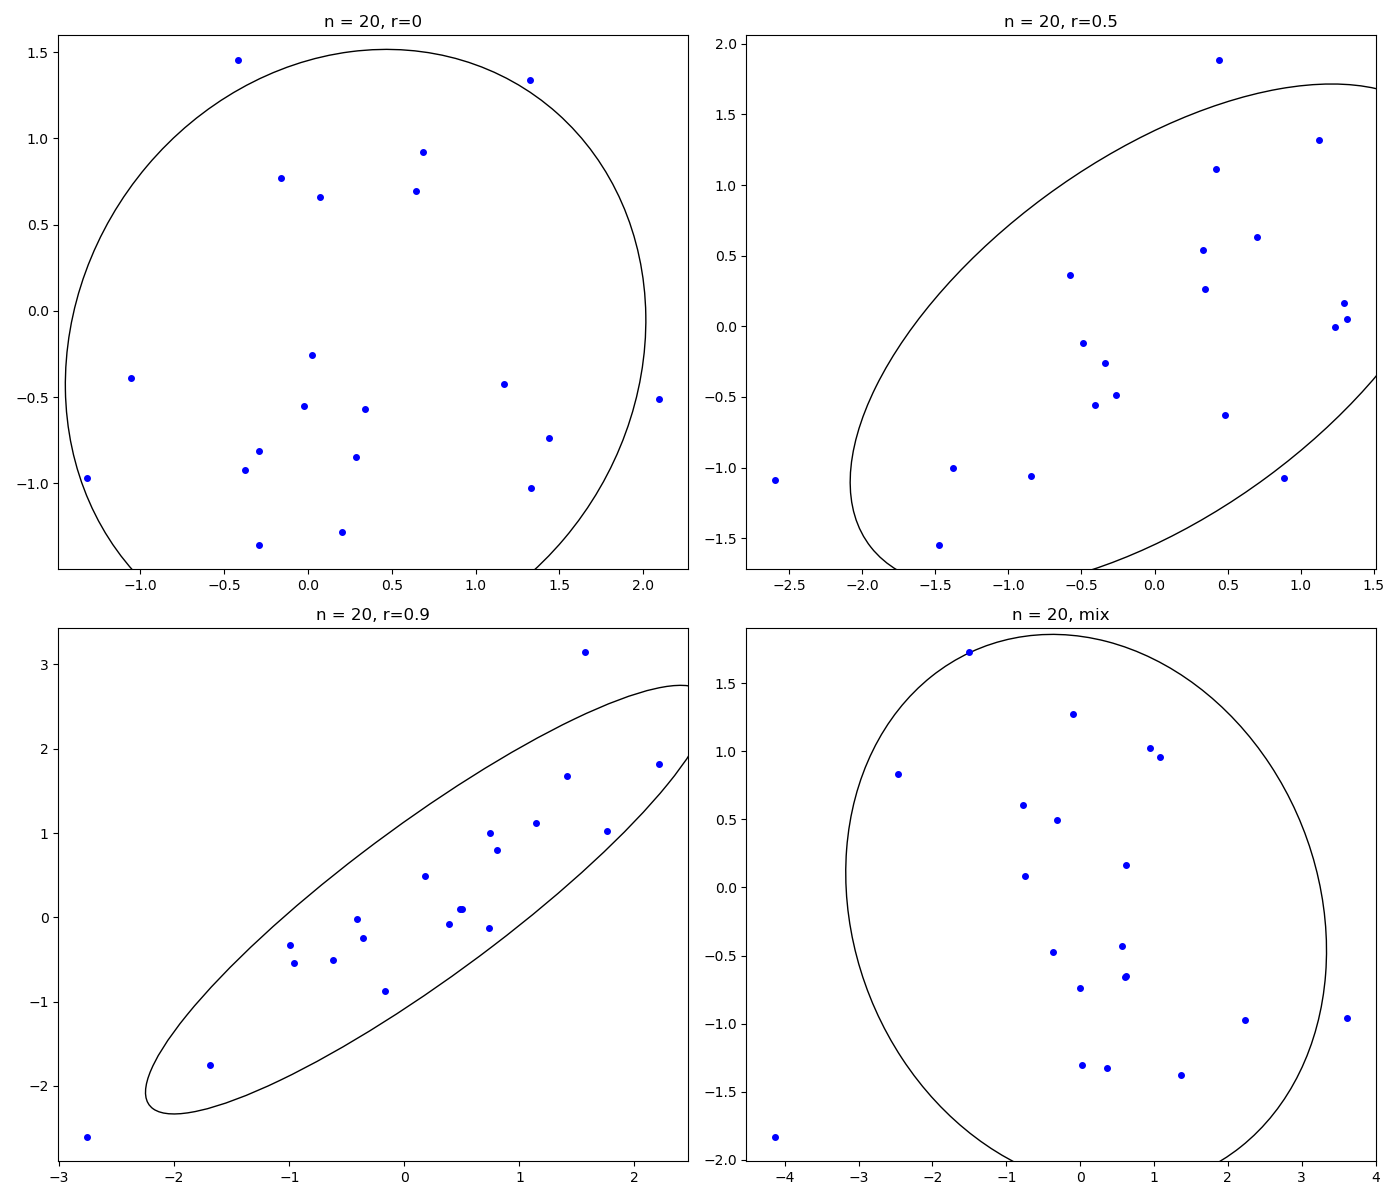
\includegraphics[scale = 0.5]{ellipse_n=20.png} 
	\label{fig:dis_norm_gis0}
\end{figure}

\vspace{-10cm}
\begin{figure}[H]
	\centering
	\caption{Графики двумерного нормального распределения и смеси для размера выборки $ n =60 $ }
	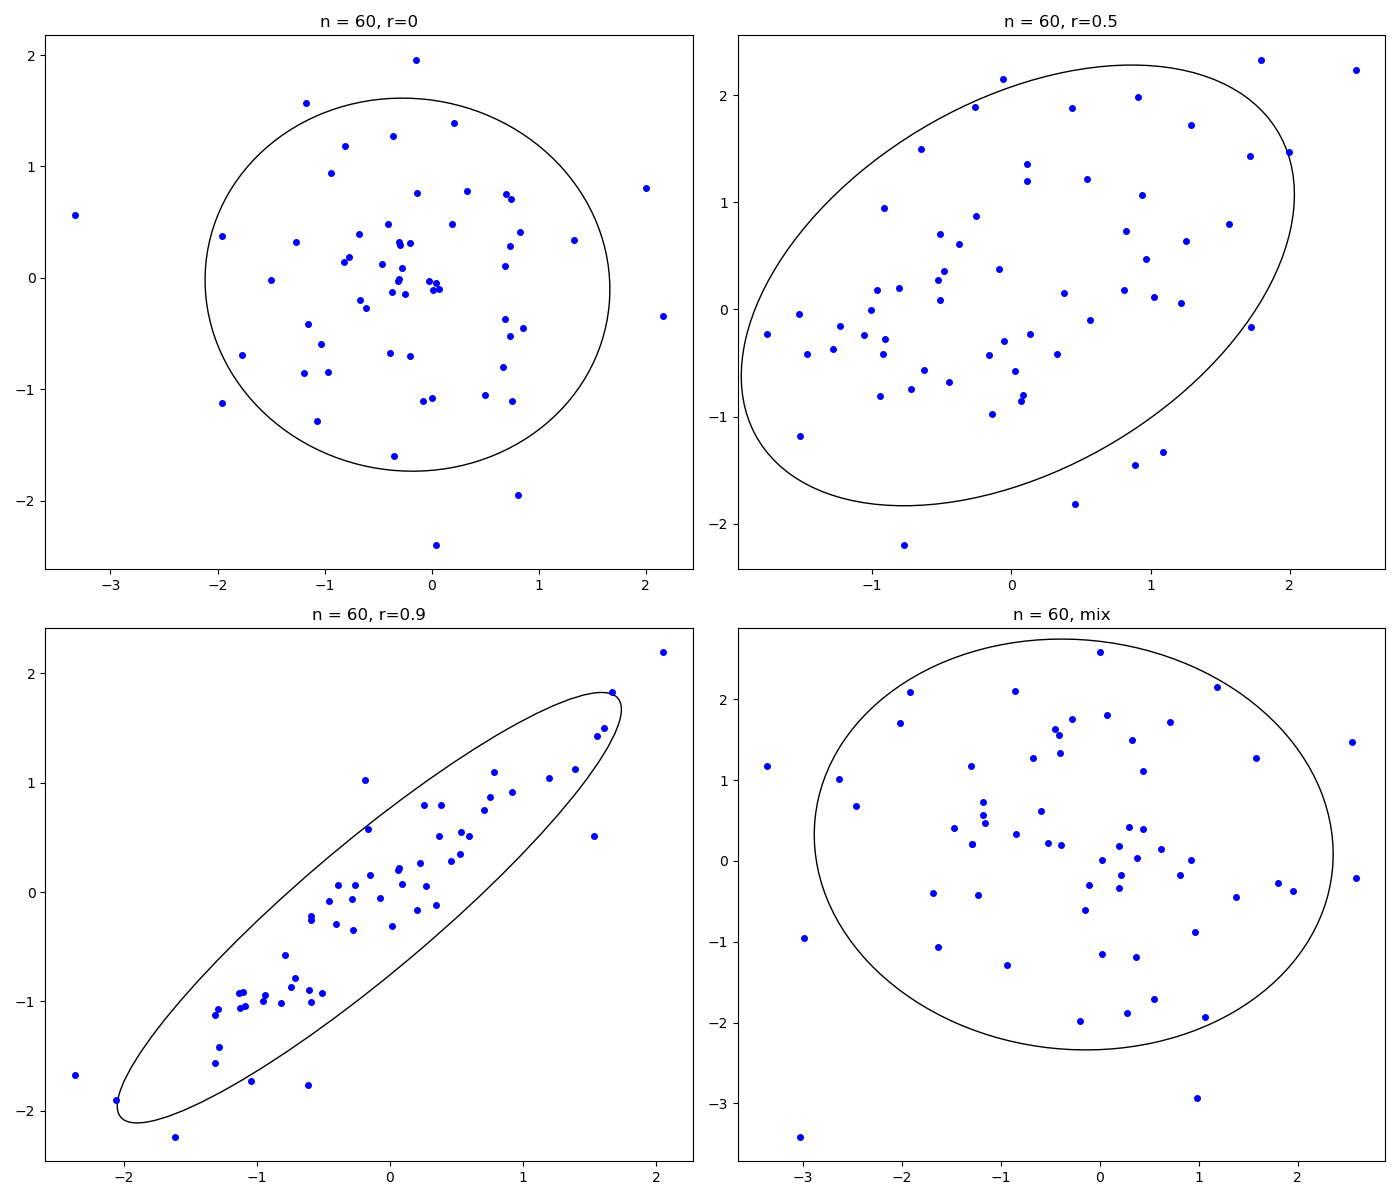
\includegraphics[scale = 0.5]{ellipse_n=60.png}
	\label{fig:dis_norm_gis1}
\end{figure}

\vspace{-1cm}
\begin{figure}[H]
	\centering
	\caption{Графики двумерного нормального распределения и смеси для размера выборки $ n =100 $ }
	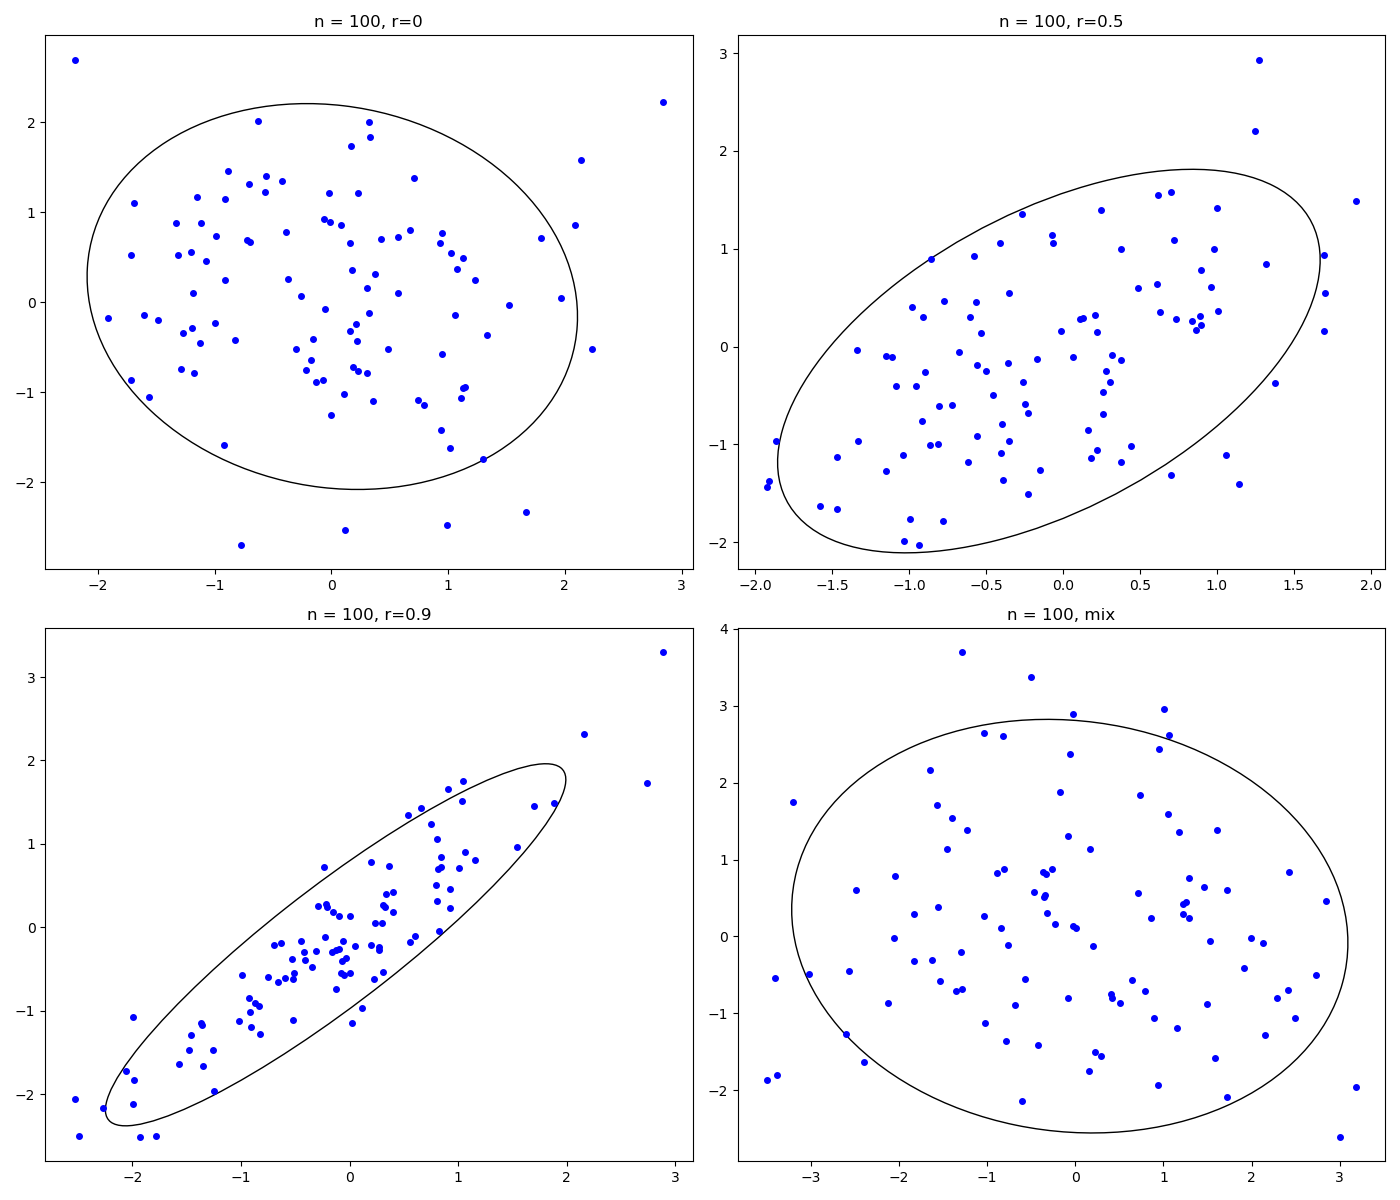
\includegraphics[scale = 0.5]{ellipse_n=100.png} 
	\label{fig:dis_norm_gis2}
\end{figure}

\begin{figure}[H]
	\centering
	\caption{Графики эллипса рассеивания для двумерного нормального распределения для $ 2 $ точек }
	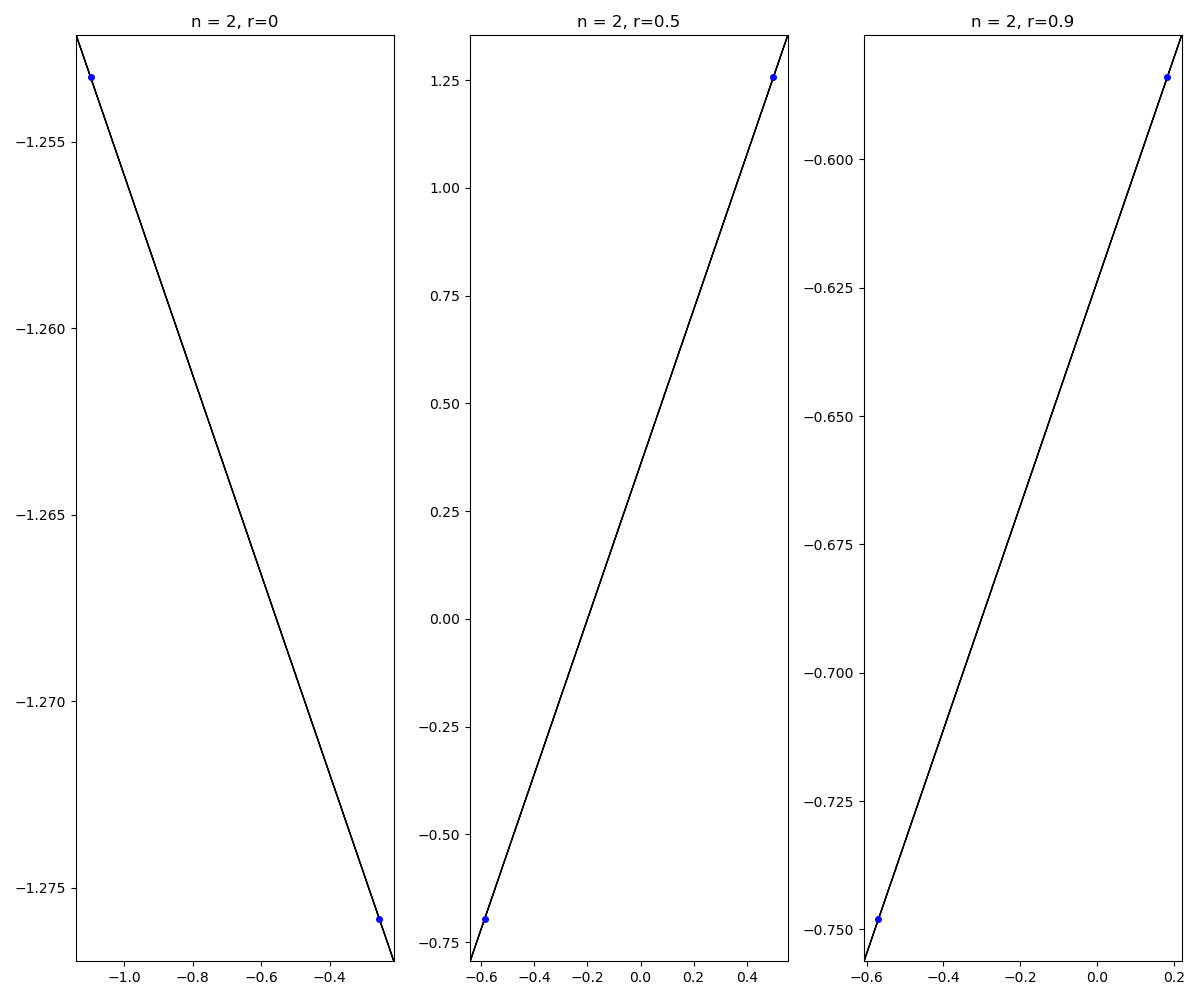
\includegraphics[scale = 0.5]{ellipse_n=2.png} 
	\label{fig:dis_norm_gis2}
\end{figure}

\begin{figure}[H]
	\centering
	\caption{Графики эллипса рассеивания для двумерного нормального распределения для $ 3 $ точек }
	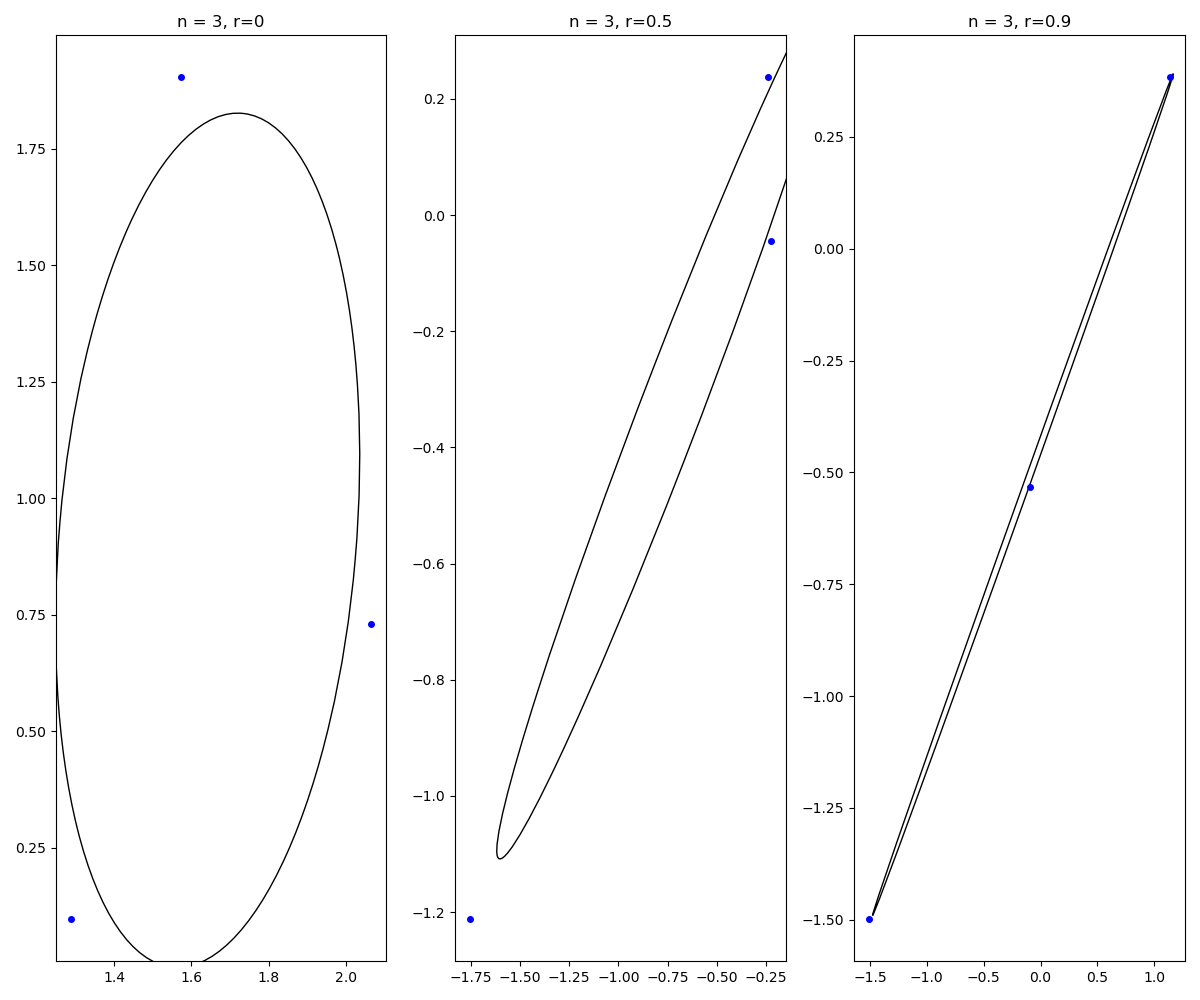
\includegraphics[scale = 0.5]{ellipse_n=3.png} 
	\label{fig:dis_norm_gis2}
\end{figure}

\subsection{Оценки линий регрессии}
%\vspace{-2cm}
\begin{figure}[H]
	\centering
	\caption{Графики линейной регрессии}
	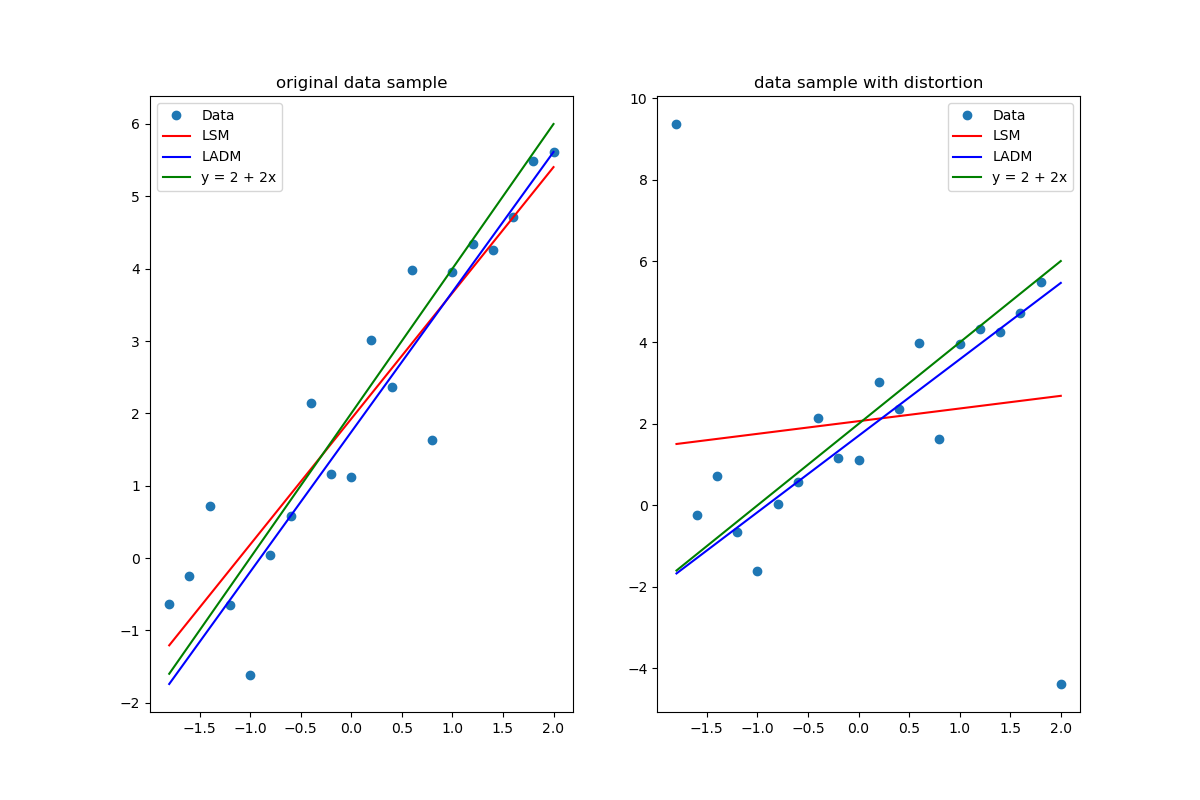
\includegraphics[scale = 0.6]{graph.png} 
	\label{fig:reg}
\end{figure}

\begin{table}[H]
	\caption{Таблица оценок коэффициентов линейной регрессии без возмущёний}
	\label{tab:my_label1}
	\begin{center}
		\vspace{5mm}
		\begin{tabular}{|c|c|c|}
			\hline
			& $\overset{\wedge}{a}$ & $\overset{\wedge}{b}$\\
			\hline
			МНК &1.739737&1.924716\\
			\hline
			МНМ &1.935446&1.742526\\
			\hline
		\end{tabular}
	\end{center}
\end{table}


\begin{table}[H]
	\caption{Таблица оценок коэффициентов линейной регрессии с возмущёниями}
	\label{tab:my_label2}
	\begin{center}
		\vspace{5mm}
		\begin{tabular}{|c|c|c|}
			\hline
			& $\overset{\wedge}{a}$ & $\overset{\wedge}{b}$\\
			\hline
			МНК &0.311165&2.067573\\
			\hline
			МНМ &1.877536 &1.707785\\
			\hline
		\end{tabular}
	\end{center}
\end{table}

\subsection{Точечная оценка параметров распределения}
\subsection{Метод максимального правдоподобия}

При подсчете оценок параметров закона нормального распределения методом максимального правдоподобия были получены следующие значения:
\begin{equation}
\begin{split}
&\overset{\wedge}{m}_{\text{МП}} = 0.090527\\
&  \overset{\wedge}{\sigma}^2_{\text{МП}} = 0.963167
\end{split}
\end{equation}
\subsection{Критерий Пирсона}
\begin{table}[H]
	\caption{Таблица вычислений $\chi^2$}
	\label{tab:my_label1}
	\begin{center}
		\vspace{5mm}
		\begin{tabular}{|c|c|c|c|c|}
			\hline
			i & $\Delta_i$ & $n_i$ & $p_i$ & $\frac{(n_i-np_i)^2}{np_i}$\\
			\hline
			1&	 $(-\infty, -1.0]$ &	15  &	 0.1288 &	 0.3501\\
			\hline
			2&	$(-1.0, -0.5)$&	10&	 0.1411&	  1.1988\\
			\hline
			3& $(-0.5, 0.0)$&	24&	 0.1927&	 1.1634\\
			\hline
			4&	$(0.0, 0.5)$&	19&	 0.2021&	 0.0721\\
			\hline
			5& $(0.5, 1.0)$&	13&	 0.1629&	 0.6626\\
			\hline
			6& $(1.0, \infty)$&	19&	 0.1725&	 0.1771\\
			\hline
			$\sum$&&		100&	1  & 3.6241	\\
			
			\hline
		\end{tabular}
	\end{center}
\end{table}

$$\chi_B^2= 3.6241$$

\subsection{Проверка гипотезы о нормальности для распределения \newline  Лапласа}
Размер выборки $ n = 25 $ для распределения Лапласа
\begin{equation}\label{eqn:laplace}
L\left( x,0,\frac{1}{\sqrt{2}}\right) = \frac{1}{\sqrt{2}}e^{-\sqrt{2}\vert x\vert}
\end{equation}
\begin{equation}
\begin{split}
&\overset{\wedge}{m}_{\text{МП}} = 0.198045\\
&  \overset{\wedge}{\sigma}^2_{\text{МП}} = 0.656187
\end{split}
\end{equation}

\begin{table}[H]
	\caption{Таблица вычислений $\chi^2$}
	\label{tab:my_label1}
	\begin{center}
		\vspace{5mm}
		\begin{tabular}{|c|c|c|c|c|}
			\hline
			i & $\Delta_i$ & $n_i$ & $p_i$ & $\frac{(n_i-np_i)^2}{np_i}$\\
			\hline
			1&	 $(-\infty, -1.0]$ &	1  &	 0.0339 &	 0.027\\
			\hline
			2&	$(-1.0, 0.0)$&	12&	 0.3475&	  1.2641\\
			\hline
			3& $(0.0, 1.0)$&	8&	 0.5078&	 1.7359\\
			\hline
			4&	$(1.0, \infty)$&	4&	 0.1108&	 0.5454\\
			\hline
			
			\hline
		\end{tabular}
	\end{center}
\end{table}

$$\chi_B^2 = 3.5725$$ 

\subsection{Интервальные оценки параметров распределения}

\begin{table}[H]
	\caption{Доверительные интервалы для параметров нормального распределения}
	\label{tab:my_label1}
	\begin{center}
		\vspace{5mm}
		\begin{tabular}{|c|c|c|}
			\hline
			& $m$ & $\sigma$\\
			\hline
			$ n = 20 $ &	 $[-0.7367, -0.0098]$ &	$ [0.5906, 1.1343] $\\
			\hline
			$ n = 100 $&	$[-0.0307, 0.356]$ & $ [0.8555, 1.1319] $\\
			\hline
		\end{tabular}
	\end{center}
\end{table}

\begin{table}[H]
	\caption{Доверительные интервалы для параметров произвольного распределения. Асимптотический подход}
	\label{tab:my_label1}
	\begin{center}
		\vspace{5mm}
		\begin{tabular}{|c|c|c|}
			\hline
			& $m$ & $\sigma$\\
			\hline
			$ n = 20 $ &	 $[-0.705, -0.0415]$ &	$ [0.6199, 1.0608] $\\
			\hline
			$ n = 100 $&	$[-0.0273, 0.3527]$& $ [0.8668, 1.1201] $\\
			\hline
		\end{tabular}
	\end{center}
\end{table}



\section{Выводы}
\subsection{Вычисление коэффициента корреляции}
По таблицам 1,2,3,4 , видно, что, при увеличении объёма выборки, подсчитанные коэффициенты корреляции стремятся к теоретическим.

Ближе всего к теоретическому коэффициенту корреляции находится коэффициент Пирсона.

По графикам также видно, что при уменьшении корреляции эллипс равновероятности стремится к окружности, а при увеличении растягивается, стремясь к прямой.

Из графиков наглядно видно, что для построения эллипса рассеивания необходимое минимальное число событий в выборке -- 3 события, так как 2 точки (2 события) вырождаются в прямую линию ( для 2 точек мы всегда можем перейти в систему координат, где у одной из компонент вектора (x,y) будет 0 мат. ожидание и 0 дисперсия, то есть переходим в одномерный случай).

\subsection{Оценки линий регрессии}
По графику \ref{fig:reg} видно, что оба метода дают хорошую оценку коэффициентов линейной регрессии, если нет выбросов. Однако выбросы сильно влияют на оценки по МНК.

Выбросы мало влияют на оценку по МНМ. Ценой за это является б\'oльшая по сравнению с МНК сложность вычисления.На практике зачастую легче просто отсеять выбросы из выборки.

\subsection{Точечная оценка параметров распределения}
Табличное значение квантиля  $\chi^2_{1-\alpha}(k-1)=\chi^2_{0.95}(5) = 11.0705$.
Полученное значение критерия согласия Пирсона для нормального распределения $\chi_B^2 = 3.6241 < \chi^2_{0.95}(5)$, следовательно основная гипотеза $H_0$ на исходной выборке не может быть отвергнута на уровне значимости $\alpha = 0.05.$. Для распределения Лапласа полученное значение критерия Пирсона $\chi_B^2 = 3.5725 < \chi^2_{0.95}(3) = 7.8147$ означает что из полученной выборки мы не можем отвергнуть гипотезу $H_0$ о нормальности исходного распределения. Такой результат легко объясним низким размером выборки, так как интервалы в которых мы оцениваем распределение получаются слишком большими, на которых распределение Лапласа очень схоже с нормальным.

\subsection{Интервальные оценки параметров распределения}

Качество оценок растёт с увеличением объёма выборки, оба метода показывают схожие точности оценки, но у ассимптотического подхода очевидно преимущество в применимости к выборке из произвольного распределения.

\section{Литература}

\href{https://physics.susu.ru/vorontsov/language/numpy.html}{Модуль numpy}

\href{https://matplotlib.org/3.1.1/api/_as_gen/matplotlib.pyplot.boxplot.html}{matplotlib boxplot}

\href{https://habr.com/ru/post/267123/}{Боксплот Тьюки}

\href{https://www.scipy.org/}{Модуль scipy}\\

\href{https://matplotlib.org/}{Модуль matplotlib}\\

\section{Приложения}

\href{https://github.com/dmitry-maltsov/PolyMatStat/blob/master/5/lab5.py}{Код 5-й лабораторной}

\href{https://github.com/dmitry-maltsov/PolyMatStat/blob/master/6/lab6.py}{Код 6-й лабораторной}

\href{https://github.com/dmitry-maltsov/PolyMatStat/blob/master/7/lab7.py}{Код 7-й лабораторной}

\href{https://github.com/dmitry-maltsov/PolyMatStat/blob/master/8/lab8.py}{Код 8-й лабораторной}

\end{document}